\documentclass[aspectratio=169]{beamer}

\usepackage[sfdefault]{FiraSans}
\usepackage{DejaVuSansMono}
\usepackage[utf8]{inputenc}
\usepackage[T1]{fontenc}

\usepackage{amsmath}
\usepackage{wasysym}

\usepackage{listings}
\usepackage{lstautogobble}
\lstset{
  autogobble,
  basicstyle=\ttfamily\footnotesize,
  keywordstyle=\color{blue},
  commentstyle=\color{gray},
  keepspaces,
  mathescape,
  escapechar=|,
  columns=fixed,
  literate={∷}{{:\!\!:}}1
           {₀}{{\textsubscript{0}}}1
           {₁}{{\textsubscript{1}}}1
           {←}{{\csname u8:\detokenize{←}\endcsname}}1
           {→}{{\csname u8:\detokenize{→}\endcsname}}1
           {↓}{{\csname u8:\detokenize{↓}\endcsname}}1
           {↑}{{\csname u8:\detokenize{↑}\endcsname}}1
}
\lstdefinestyle{cpp}{
  language=c++,
  morekeywords={decltype}
}
\lstdefinestyle{haskell}{
  morecomment=[l]{--},
  morekeywords={data,type}
}
\lstnewenvironment{cppcode}{\lstset{style=cpp}}{}
\lstnewenvironment{haskellcode}{\lstset{style=haskell}}{}
\newcommand{\cppinline}[1]{\lstinline[style=cpp]|#1|}
\newcommand{\haskellinline}[1]{\lstinline[style=haskell]|#1|}

\newcommand{\halcheck}{\texttt{\footnotesize{halcheck}}}

\title{\halcheck}
\author{Anthony Vandikas}
\date{December 22, 2023}
\usetheme{metropolis}

\begin{document}

\frame{\titlepage}

\begin{frame}{\halcheck{} --- Overview}
  \tableofcontents
\end{frame}

\section{Overview}

\begin{frame}<1>[label=overview]{\halcheck{} --- Overview \only<4>{--- Summary}}
  \begin{block}{Why \halcheck?}
    \begin{enumerate}
      \item<alert@1> First-order(ish) API
      \item<alert@2> Support for custom test-case generation strategies
      \item<alert@3> Better space complexity
    \end{enumerate}
  \end{block}
\end{frame}

\begin{frame}[fragile]{\halcheck{} --- Overview --- API}
  All PBT frameworks are direct ports or descendants of QuickCheck. These frameworks all consist of:

  \bigskip{}
  \pause{}

  \begin{columns}[T,onlytextwidth]
    \begin{column}{0.47\textwidth}
      \begin{block}{A central generator data type:}
        \begin{haskellcode}
          --     Source of
          --     randomness ↓
          data Gen a = Gen (Random → a)
        \end{haskellcode}
      \end{block}
    \end{column}

    \pause{}

    \begin{column}{0.53\textwidth}
      \begin{block}{A set of basic combinators:}
        \begin{haskellcode}
          choose    ∷ (Int, Int) → Gen Int
          suchThat  ∷ (a → Bool) → Gen a → Gen a
          frequency ∷ [(Int, Gen a)] → Gen a
          ...
        \end{haskellcode}
      \end{block}
    \end{column}
  \end{columns}

  \pause{}

  \bigskip{}

  \begin{itemize}
    \item Users must be comfortable reasoning about higher-order functions.
    \item Users must ensure generators are only invoked in the \alert{correct context}.
  \end{itemize}
\end{frame}

\begin{frame}[fragile,t]{\halcheck{} --- Overview --- API}
  \textbf{Example:} \emph{Write a generator combinator that produces \cppinline{std::vector}s up to (but not including) a given length.}

  \begin{onlyenv}<+>
    \begin{cppcode}
      // RapidCheck
      Gen<std::vector<int>> example(int N) {
        return gen::container<std::vector<int>>(
          *gen::inRange(0, N),
          gen::arbitrary<int>);
      }
    \end{cppcode}

    \begin{haskellcode}
      -- QuickCheck
      example n = vectorOf (choose (0, n - 1)) arbitrary
    \end{haskellcode}
  \end{onlyenv}

  \begin{onlyenv}<+>
    \begin{cppcode}
      // RapidCheck
      Gen<std::vector<int>> example(int N) {
        return gen::container<std::vector<int>>(
          *gen::inRange(0, N), // WRONG (no compiler error)
          gen::arbitrary<int>);
      }
    \end{cppcode}

    \begin{haskellcode}
      -- QuickCheck         ↓ WRONG (compiler error)
      example n = vectorOf (choose (0, n - 1)) arbitrary
    \end{haskellcode}
  \end{onlyenv}

  \begin{onlyenv}<+>
    \begin{cppcode}
      // RapidCheck
      Gen<std::vector<int>> example(int N) {
        // WRONG: n is computed $\mathbf{once}$, $\mathit{before}$ calling container
        auto n = *gen::inRange(0, N);
        return gen::container<std::vector<int>>(n, gen::arbitrary<int>());
      }
    \end{cppcode}
    \begin{haskellcode}
      -- QuickCheck         ↓ WRONG: choose ∷ (Int, Int) → $\color{red}{\mathtt{Gen\ Int}}$
      example n = vectorOf (choose (0, n - 1)) arbitrary
      --          ↑ WRONG: vectorOf ∷ $\color{red}{\mathtt{Int}}$ → Gen Int → Gen [Int]
    \end{haskellcode}
  \end{onlyenv}

  \begin{onlyenv}<+>
    \textbf{Solution:} Delay computation of \cppinline{*gen::inRange(0, N)} using \cppinline{gen::exec}.

    \begin{columns}[T,onlytextwidth]
      \column{0.53\textwidth}
      \begin{cppcode}
        // RapidCheck
        Gen<std::vector<int>> example(int N) {
          return gen::exec([=] {
            return *gen::container<std::vector<int>>(
              *gen::inRange(0, N),
              gen::arbitrary<int>);
          });
        }
      \end{cppcode}

      \column{0.35\textwidth}
      \begin{haskellcode}
        -- QuickCheck
        example n = do
          i <- choose (0, n - 1)
          vectorOf i arbitrary
      \end{haskellcode}
    \end{columns}
  \end{onlyenv}
\end{frame}

\begin{frame}[fragile]{\halcheck{} --- Overview --- API}
  \begin{itemize}
    \item \textbf{Problem:} Need to ensure generators are only invoked in the correct context.
          \begin{itemize}
            \item Haskell's type system ensures this always happens.
            \item C++'s type system can provide no such guarantee!
          \end{itemize}
          \pause{}
    \item \textbf{Solution:} Get rid of the generator type!
          \begin{itemize}
            \item All code is written in the generator context.
            \item Bonus: fewer higher-order functions.
          \end{itemize}
  \end{itemize}

  \begin{cppcode}
    // halcheck
    std::vector<int> example(int N) {
      return gen::container<std::vector<int>>(
        gen::range(0, N),
        gen::arbitrary<int>);
    }
  \end{cppcode}
\end{frame}

\againframe<2>{overview}

\begin{frame}{\halcheck{} --- Overview --- Strategies}
  There are various desirable strategies for generating data:
  \begin{itemize}
    \item Random (almost everything)
    \item Enumerative (SmallCheck/LeanCheck) \pause{}
    \item Learning-based (RLCheck)
    \item Coverage-guided (FuzzTest) \pause{}
  \end{itemize}

  Most PBT frameworks (and all C++ PBT frameworks) use a \alert{fixed strategy}.
\end{frame}

\begin{frame}[fragile]{\halcheck{} --- Overview --- Strategies}
  \halcheck{} provides combinators for specifying strategies:

  \begin{cppcode}
    //   random(int) → strategy
    // ↓ Executes random test cases forever or until a bug is found.
    test::random(seed)([] { /* test code */ });
  \end{cppcode}

  \pause{}

  \begin{cppcode}
    //   ordered(strategy) → strategy
    // ↓ Executes all test cases in order, from smallest to largest.
    test::ordered()([] { /* test code */ });
  \end{cppcode}

  \pause{}

  \begin{cppcode}
    //   limit(strategy, int) → strategy
    //   shrink(strategy) → strategy
    //   Executes at most 100 random test cases.
    // ↓ Performs shrinking if an exception is thrown.
    test::shrink(test::limit(test::random(), 100))([] { /* test code */ });
  \end{cppcode}

  \pause{}

  (Intended for advanced users.)
\end{frame}

\againframe<3>{overview}

\begin{frame}[fragile]{\halcheck{} --- Overview --- Space Complexity}
  \begin{columns}[t,onlytextwidth]
    \column{0.5\textwidth}
    \begin{block}{How does shrinking work?}
      \bigskip

      Internally, every generator is a function returning a ``shrink tree'' of values.

      \bigskip

      \begin{haskellcode}
        data Gen a = Gen (Random → Tree a)
      \end{haskellcode}

      Shrink trees can be \alert{very large} so they must be computed lazily.
    \end{block}

    \column{0.5\textwidth}
    \begin{block}{Shrink tree for a list:}
      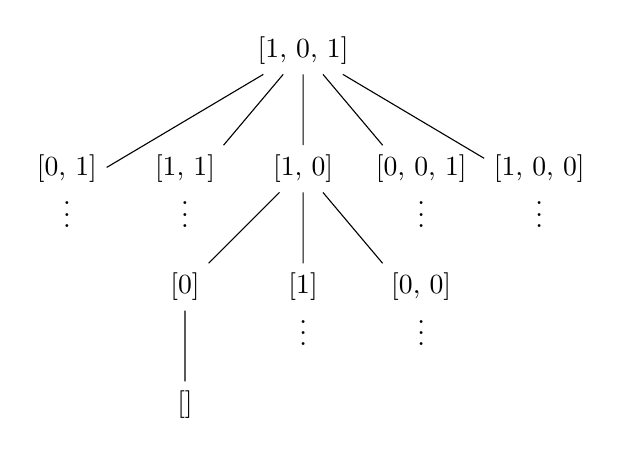
\begin{tikzpicture}[align=center,anchor=north,level distance=1.2cm]
        \node{[1, 0, 1]}
        child {node {[0, 1]\\\vdots}}
        child {node {[1, 1]\\\vdots}}
        child {node {[1, 0]}
            child {node {[0]}
                child {node {[]}}}
            child {node {[1]\\\vdots}}
            child {node {[0, 0]\\\vdots}}}
        child {node {[0, 0, 1]\\\vdots}}
        child {node {[1, 0, 0]\\\vdots}}
        ;
      \end{tikzpicture}
    \end{block}
  \end{columns}

  \pause{}

  This implementation strategy \alert{does not work for C++!}
\end{frame}

\begin{frame}[fragile]{\halcheck{} --- Overview --- Space Complexity}
  \begin{block}{Example:}
    \begin{cppcode}
      auto xs = *gen::arbitrary<std::vector<int>>();
      auto x  = *gen::elementOf(xs);
    \end{cppcode}
  \end{block}

  \pause{}

  \begin{itemize}
    \item To shrink \cppinline{x}, RapidCheck must pick a different element of \cppinline{xs}.
          \pause{}

    \item Shrinking is performed \emph{after} the test case has finished (\alert{\cppinline{xs} no longer exists})!
          \begin{itemize}
            \item Not a problem in languages with automatic memory management.
          \end{itemize}
          \pause{}

    \item \cppinline{gen::elementOf} must store a copy of \cppinline{xs} in order to avoid creating a dangling reference.
          \pause{}
  \end{itemize}

  \textbf{Conclusion:} all combinators (with shrinking behaviour) must make copies of their arguments!

  \pause{}

  \textbf{Problem:} by default, copies in C++ are deep ($\mathcal{O}(n)$ instead of $\mathcal{O}(1)$).
\end{frame}

\begin{frame}[fragile]{\halcheck{} --- Overview --- Space Complexity}
  \begin{block}{Generators cannot return references:}
    \begin{cppcode}
      // Generates a random reference
      // to an element of xs.
      rc::Gen<int &> referenceOf(??? xs);
      //          What goes here? ↑

      // Example: assign a
      // random element to 0.
      *referenceOf(xs) = 0;
    \end{cppcode}

    What type should \cppinline{referenceOf} have?
  \end{block}
\end{frame}

\begin{frame}{\halcheck{} --- Overview --- Space Complexity}
  \cppinline{halcheck} is inspired by work on \alert{internal shrinking}.
  \begin{itemize}
    \item Motto: shrink inputs, not outputs!
    \item Data is recomputed, never copied.
  \end{itemize}

  \pause{}

  \textbf{Note:} \cppinline{halcheck} does \alert{not} use internal shrinking.
  \begin{itemize}
    \item Users have full control over shrinking.
  \end{itemize}
\end{frame}

\againframe<4>{overview}

% In this section I will go over the design of halcheck. I will
% 1. go through each design goal,
% 2. explain the motivation behind each goal (if I haven't already), and
% 3. explain how halcheck fulfils that goal, with examples.
\section{Design}

\begin{frame}[t,fragile]{\halcheck{} --- Design}
  % Goal: we want a simple API with few higher-order functions and no generator type.
  % This is a central design choice for the library.
  % I've already explained why we want this in the previous part.
  \textbf{Goal:} Simple API with few higher-order functions and no generator type.\\

  \begin{columns}[onlytextwidth]
    \column{0.65\textwidth}
    \begin{cppcode}
      template<typename T>
      T gen::arbitrary();

      template<typename T>
      T gen::range(T min, T max);

      template<typename T>
      T &gen::element(std::vector<T> &container);

      template<typename T, typename F>
      T gen::container<T>(size_t size, F gen);
    \end{cppcode}

    % We want users to define generators by "just" writing normal functions.
    \column<2>{0.35\textwidth}
    \centering\Large Motto:\\\alert{Just write functions!}
  \end{columns}
\end{frame}

\begin{frame}[t,fragile]{\halcheck{} --- Design --- Core}
  % To achieve our goal of a simple first-order, generator-less API,
  % halcheck provides a function, gen::next.
  \textbf{Goal:} Simple API with few higher-order functions and no generator type.
  \begin{center}
    \cppinline{bool gen::next(int w₀, int w₁);}
  \end{center}

  \begin{overprint}
    % This is halcheck's *only* source of randomness.
    % All generators are built from this function.
    % All it does is perform a weighted coin flip.
    \onslide<2,3>
    \begin{itemize}
      \item Returns \cppinline{true} with probability $\frac{w_1}{w_0 + w_1}$ ($w_0$ and $w_1$ are relative weights).
      \item<3> This is the \alert{only} source of randomness --- all generators are built from this function!
    \end{itemize}

    % Here's an example of how we can use this function to define a generator for a range.
    % This is basically a binary search, except we perform a coin flip instead of a comparison.
    % The size of the range can be odd, we need to use a weighted coin flip to ensure uniformity.
    % Notice the TODO in the case min >= max -- I'll get to this in a moment.
    \onslide<4>
    \vspace{-1em}
    \begin{block}{Example:}
      \begin{cppcode}
      int gen::range(int min, int max) {
        while (min + 1 < max) {
          auto mid = std::midpoint(min, max);
          if (|\alert{gen::next}|(mid - min, max - mid))
            max = mid;
          else
            min = mid; }
        return min; }
    \end{cppcode}
    \end{block}
  \end{overprint}
\end{frame}

\begin{frame}[t,fragile]{\halcheck{} --- Design --- Core}
  % A weighted coin toss is all we need to compute random data.
  % But users expect a lot more from a property-based testing library.
  % If we had a central generator type, we could support them all just by extending this type.
  % * For sized generation, just add an extra parameter
  % * For shrinking, change the output to a shrink tree
  % * For reporting distributions, add a list of labels to the output
  % * If we want the ability to discard test-cases, just make the output optional.
  \begin{columns}[onlytextwidth]
    \column{0.5\textwidth}
    \begin{block}{Users expect more!}
      \begin{itemize}
        \item<2-|alert@2,7> Discards
        \item<3-|alert@3,8> Sized generation
        \item<4-|alert@4,9> Distribution logging
        \item<5-|alert@5,10> Shrinking
      \end{itemize}
    \end{block}

    \column{0.5\textwidth}
    \begin{haskellcode}
      data Gen a = Gen
        ( Random|\only<3->{\\\ \ → \alert<3>{Size}}|
        → |\only<2->{\alert<2>{Maybe} }||\only<4->{(}||\only<5->{\alert<5>{Tree} }|a|\only<4->{, \alert<4>{[Label]})}|
        )
    \end{haskellcode}
  \end{columns}

  % In halcheck we've committed to a "generator-less" interface.
  % There is no generator type to extend!
  % How can we support all these features by only providing functions?
  \onslide<6->
  What \alert{functions} do we need to provide to support these features?

  \begin{columns}[onlytextwidth]
    \column{0.45\textwidth}
    \begin{itemize}
      \item<7->[\alert<7>{\textbullet}] \cppinline{void gen::discard()} \only<7>{\\(throws exception)}
      \item<9->[\alert<9>{\textbullet}] \cppinline{void gen::label(std::string)}
    \end{itemize}
    \column{0.55\textwidth}
    \begin{itemize}
      \item<8->[\alert<8>{\textbullet}] \cppinline{int gen::size()}
      \item<10->[\alert<10>{\textbullet}] \cppinline{???}
    \end{itemize}
  \end{columns}
\end{frame}

\begin{frame}[fragile,t]{\halcheck{} --- Design --- Core --- \cppinline{gen::shrink}}
  \begin{center}
    \cppinline{std::optional<int> gen::shrink(int size = 1)}
  \end{center}

  \begin{overprint}
    \onslide<+>
    \begin{itemize}
      \item \cppinline{gen::shrink(n)} returns an \cppinline{int i} if shrinking should occur at the call site, and \cppinline{std::nullopt} otherwise.
      \item Intuitively, \cppinline{i} is the \emph{index} of the child element to shrink to.
    \end{itemize}

    \onslide<+->
    \begin{columns}[T]
      \column{0.48\textwidth}
      \begin{block}{Example:}
        \begin{cppcode}
          std::string gen_string() {
            auto xs = /* random string */;
            for (size_t i = 0; i < xs.size();)
              if (auto c = |\alert{gen::shrink}(2)|) $\only<.(2)>{\alert{\Longleftarrow}}$
                if (*c == 0) xs.erase(i); $\only<.(3)>{\alert{\Longleftarrow}}$
                else         xs[i] = '\0'; $\only<.(4)>{\alert{\Longleftarrow}}$
              else $\only<.(1)>{\alert{\Longleftarrow}}$
                i++;
            return xs; }
        \end{cppcode}
      \end{block}

      \column{0.52\textwidth}
      \begin{block}{Explanation:}
        \begin{enumerate}
          \item<+-|alert@+> Normally, \cppinline{gen::shrink(n)} always returns \cppinline{nullopt}, so \cppinline{xs} is unmodified.
          \item<+-|alert@+> When shrinking, \cppinline{gen::shrink(n)} returns an integer $c < n$.
            \begin{enumerate}
              \item<+-|alert@+> If $c = 0$: remove current element.
              \item<+-|alert@+> If $c = 1$: shrink current element to 0.
            \end{enumerate}
        \end{enumerate}
      \end{block}
    \end{columns}
  \end{overprint}
\end{frame}

\begin{frame}[fragile,t]{\halcheck{} --- Design --- Core --- \cppinline{gen::shrink}}
  \begin{itemize}
    \item \cppinline{gen::shrink} provides a minimal interface for defining shrinking behaviour.
    \item Not meant to be used directly!
    \item Other combinators (e.g., Hedgehog's \haskellinline{shrink}) can be built using \cppinline{gen::shrink}.
  \end{itemize}

  \begin{center}
    But \cppinline{gen::shrink} has a problem!
  \end{center}
\end{frame}

\begin{frame}[fragile,t]{\halcheck{} --- Design --- Core --- \cppinline{gen::shrink}}
  \begin{columns}[T]
    \column{0.4\textwidth}
    \begin{overprint}
      \textbf{Example:}

      \onslide<1-7>
      \begin{cppcode}
        gen::next → |\color{violet}{true}|, |\color{red}{false}|, |\color{olive}{true}|

        int x = 0;
        if (|\only<1>{gen::next()}\only<2->{\textcolor{violet}{true}}| && |\only<1-2>{!gen::shrink()}\only<3->{\textcolor{blue}{false}}|)
          x += |\only<1>{gen::next()}\only<2-5>{\textcolor{red}{false}}\only<6->{\textcolor{gray}{gen::next()}}| ? 1 : 0;
        x += |\only<1>{gen::next()}\only<2-6>{\textcolor{olive}{true}}\only<7>{\textcolor{red}{false}}| ? 1 : 0;
      \end{cppcode}

      \onslide<8->
      \begin{cppcode}
        gen::next → [|\color{violet}{true}|, |\color{red}{false}|], |\color{olive}{true}|

        int x = 0;
        {
          auto _ = |\alert{gen::group}|();
          if (|\only<8>{gen::next()}\only<9->{\textcolor{violet}{true}}| && |\only<8-9>{!gen::shrink()}\only<10->{\textcolor{blue}{false}}|)
            x += |\only<8>{gen::next()}\only<9>{\textcolor{red}{true}}\only<10>{\textcolor{gray}{gen::next()}}| ? 1 : 0;
        }
        x += |\only<8>{gen::next()}\only<9->{\textcolor{olive}{true}}| ? 1 : 0;
      \end{cppcode}
    \end{overprint}

    \column{0.6\textwidth}
    \begin{overprint}
      \onslide<1-4>
      \textbf{Explanation:}
      \begin{itemize}
        \item<2-> Suppose a test case failure occurs.
        \item<3-> Then \cppinline{!gen::shrink()} subsequently evaluates to \cppinline{false}.
        \item<4-> Final call to \cppinline{gen::next} should return the same value (\texttt{\footnotesize\color{olive}{true}}).
      \end{itemize}

      \onslide<5-7>
      \textbf{Problem:}
      \begin{itemize}
        \item<5-> \halcheck{} is just a library. It can't inspect the internal structure of a program!
        \item<5-> Internally, \halcheck{} only saves and replays the results of \cppinline{gen::next}.
        \item<6-> Second call to \cppinline{gen::next} is never evaluated.
        \item<7-> Final call to \cppinline{gen::next} returns next available value (\texttt{\footnotesize\color{red}{false}})!
      \end{itemize}

      \onslide<8->
      \textbf{Solution:} \cppinline{gen::group}
      \begin{itemize}
        \item<8-> \cppinline{gen::group} informs \halcheck{} that all subsequent calls to \cppinline{gen::next} (and \cppinline{gen::shrink}) should be treated as a single ``step''.
        \item<9-> Evaluation before shrinking is unchanged.
        \item<10-> Final call to \cppinline{gen::next} returns the proper value even after shrinking!
      \end{itemize}
    \end{overprint}
  \end{columns}
\end{frame}

\begin{frame}[fragile,t]{\halcheck{} --- Design --- Core --- \cppinline{gen::group}}
  When to use \cppinline{gen::group}?
  \begin{itemize}
    \item Number of calls to \cppinline{gen::group}, \cppinline{gen::next}, and \cppinline{gen::shrink} (excluding calls within a \cppinline{gen::group}) must be \alert{constant}.
    \item Simple heuristic: wrap all conditionals and loops in a \cppinline{gen::group}.
    \begin{itemize}
      \item Future work: automatic \cppinline{gen::group} insertion via instrumentation.
    \end{itemize}
    \item Incorrect grouping will \emph{not} break tests, only cause inefficient shrinking.
  \end{itemize}
\end{frame}

\begin{frame}[fragile]{\halcheck{} --- Design --- Effects}
  \begin{itemize}
    \item All generators are implemented using the six (and counting) core functions:
          \begin{itemize}
            \item \cppinline{gen::next}
            \item \cppinline{gen::discard}
            \item \cppinline{gen::size}
            \item \cppinline{gen::label}
            \item \cppinline{gen::shrink}
            \item \cppinline{gen::group}
          \end{itemize}
    \item How are the core functions themselves implemented?
          \pause{}
          \alert{It depends!}
    \item Behaviour differs depending on strategy (e.g., random vs exhaustive).
    \item Sometimes users need to override behaviour (e.g., disable shrinking).
    \item \halcheck{} lets you \alert{override} core functions!
  \end{itemize}
\end{frame}

\begin{frame}{\halcheck{} --- Design --- Effects}
  \halcheck{}'s core functions are implemented using a primitive system of \alert{effect handlers}.

  \begin{itemize}
    \item<2-> Every core function \cppinline{f} is an \emph{effect}.
    \item<3-> A \emph{handler} \cppinline{h} for \cppinline{f} can be \emph{installed} using \cppinline{auto _ = f.handle(h)}.
    \item<4-> Handlers are \emph{uninstalled} when the return value (\cppinline{_}) goes out of scope.
    \item<5-> Effects are \emph{invoked} via the call operator (\cppinline{f()}) and behave according to the last handler that was installed.
    \item<6-> Effects are \alert{lexically scoped}: any effects invoked within an effect handler behave as if they were invoked \emph{just before the effect handler was installed}.
  \end{itemize}
\end{frame}

\begin{frame}[fragile]{\halcheck{} --- Design --- Effects}
  \textbf{Example:} Overriding \cppinline{gen::next}
  \begin{cppcode}
    CHECK_THROWS(gen::next()); // Throws by default
    {
      //   ↓ gen::next calls the lambda as long as this is in scope
      auto _ = gen::next.handle([](int x, int y) {
        CHECK_THROWS(gen::next()); // Calling gen::next within the handler
                                   // invokes the previous behaviour.
        return x == 0 && y > 0;
      });
      CHECK_EQ(gen::next(0, 1), true);
    }
    CHECK_THROWS(gen::next()); // Original behaviour restored
  \end{cppcode}
\end{frame}

\section{Summary}

\begin{frame}{\halcheck{} --- Design --- Summary}
  \begin{itemize}
    \item Every generator in \halcheck{} is built from four first-order core functions, enabling a "direct-style" API.
    \item User-defined generation strategies are supported: every core function can be overriden.
    \item Shrinking is performed by changing generator inputs (\mintinline{c++}{gen::shrink}) instead of generator outputs, resulting in less memory usage.
  \end{itemize}
\end{frame}


\end{document}
